\section{Development method}

The devlopment method used will be the conventional Waterfall model. The Waterfall model works well whenever everything goes according to plan, however in a complex project problems are bound to appear. Thus it is important to perfect the specification before attempting to execute it.
\begin{figure}[h]
	\centering
	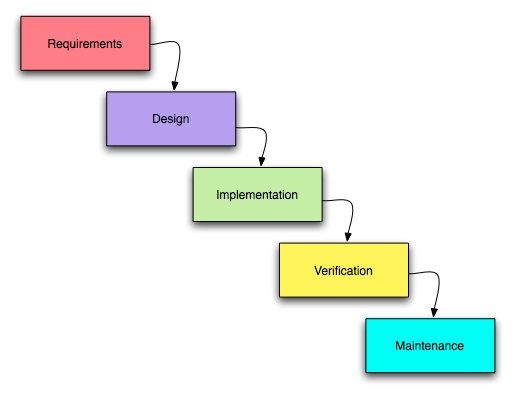
\includegraphics[width=0.5\textwidth]{Images/development_method_waterfall_model.png}
	\caption{Waterfall model}
	\label{Waterfall}
\end{figure}

In the Waterfall model, the following phases are followed in order:
\begin{enumerate}
\item Requirements specification (Requirements analysis)
\item Software design
\item Implementation and Integration
\item Testing (or Validation)
\item Deployment (or Installation)
\item Maintenance
\end{enumerate}

\begin{figure}[h]
	\centering
	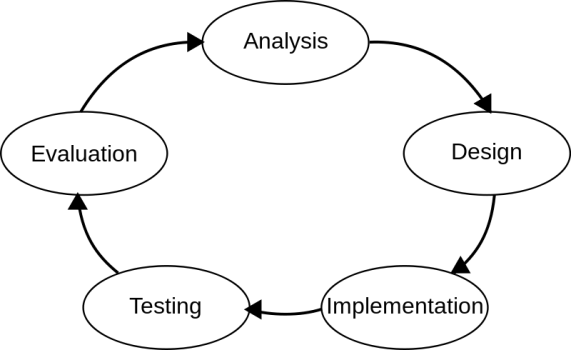
\includegraphics[width=0.5\textwidth]{Images/development_method_software_development_cycle.png}
	\caption{Software Development cycle l}
	\label{cyclel}
\end{figure}

Software Development cycle 
